\documentclass[pdftex,10pt,a4paper,oneside]{article}
%Can change the pt, papersize etc.
\usepackage{listings}
\usepackage{amsmath}
\usepackage{amssymb}
\usepackage{algorithm}
\usepackage{algorithmic} %Algorithm styles, need to be nested for the example shown
\usepackage{fancyhdr} %For our headers
\usepackage{graphicx} %Inserting images
\usepackage{lipsum}  %Blank text fill, delete me when finished
\usepackage{setspace} %Spacing on the front page for crest and titles
\usepackage[]{fncychap} % Styles can be Sonny, Lenny, Glenn, Conny, Rejne, Bjarne and Bjornstrup
\usepackage[hyphens]{url} %Deals with hyphens in urls to make them clickable
\usepackage{xcolor} %Great if you want coloured text
\usepackage{tabularx}
\usepackage{appendix} %Take a wild guess slick

%KEEP THIS ONE LAST it's quite buggy, it allows you to click on links within the pdf and web links without changing the colour. The mouse cursor simply changes its icon to indicate to the user. Great tool - still awkward
\usepackage[hidelinks]{hyperref}


%This will tell the compiler to do the header style, page and spacing between the header and text
\fancyhf{}
\renewcommand{\headrulewidth}{0.2pt}




% Load the package
\usepackage[toc]{glossaries}

% Generate the glossary
\makeglossaries
%\includeonly{%chapters/ch1.tex,
%	chapters/ch3.tex,
%	chapters/ch4.tex,
%	chapters/ch5.tex,
%	chapters/ch6.tex,
	%chapters/ch7.tex,
	%chapters/ch8.tex,
	%chapters/ch9.tex,
	%chapters/ch10.tex,
%	chapters/ch11.tex,
%	chapters/ch12.tex,
	%chapters/ch13.tex,	}
\begin{document}
	
	\pagenumbering{arabic}
	
	\begin{spacing}{2}
		\begin{center}
			
\includegraphics[scale = 0.20]{ASU.png}
		\end{center}
		\vspace{5mm}
		\begin{center}
			\textbf{\begin{LARGE}
					MultiMedia Retrieval
			\end{LARGE}}
			\vspace{2mm}
		\end{center}
		\begin{center}
			\textbf{\large Ahmed Maged Abdel almonem\\Ahmed Mohammed Ibrahim\\ Bassem Mohamed Yousry\\Mohamed Atta Ibrahim \\Mahmoud Mohamed Benyamin\\Mahmoud Othman Rabee \\ Hady Ashraf Ragab\\Yousef Abdelbadea Ali}
			\vspace{2mm}
		\end{center}
		\begin{center}
			\textbf{\large Supervisor: Dr. Gamal A Ebrahim }\\
			\textbf{\large Department of Computer and Systems Engineering}\\
			\textbf{\large Faculty of Engineering at Ain Shams University}\\
			
			{\large \today\\}
		\end{center}
	\end{spacing}
	
	\pagebreak
	
	\tableofcontents
	\pagebreak
	\listoffigures
	\pagebreak
	\listoftables
	\pagebreak
	\begin{abstract}{
			This paper presents imp multimedia project
	}	\end{abstract}
	\pagebreak
	\section*{Introduction}
	During this project, we will use multimedia techniques to analyze, design, and implement a content-based multimedia retrieval system, with images and videos as the two media that we will use. In addition, by the end of the project, we had generated code that showed the project's extensive analysis, design, and testing, as well as a description of the methodologies used, a problem description, detailed solution, limitations, sample output, references, and any other relevant information.
	 
	\addcontentsline{toc}{section}{Introduction}
	
	
	\pagebreak
	
	\section{project description}
	This is a python desktop application, it applies the multimedia techniques to analyze, design, and implement content-based multimedia retrieval system, where the two media that we are going to use are the images and the videos. In CBIR we have implemented three techniques color based using color histogram, texture based using gabour filter and shape based using histogram of gradient, in CBVR we used two techniques. the key frames extraction technique and content-based technique (Closed Captions).
	\begin{figure}[H]
		\centering
		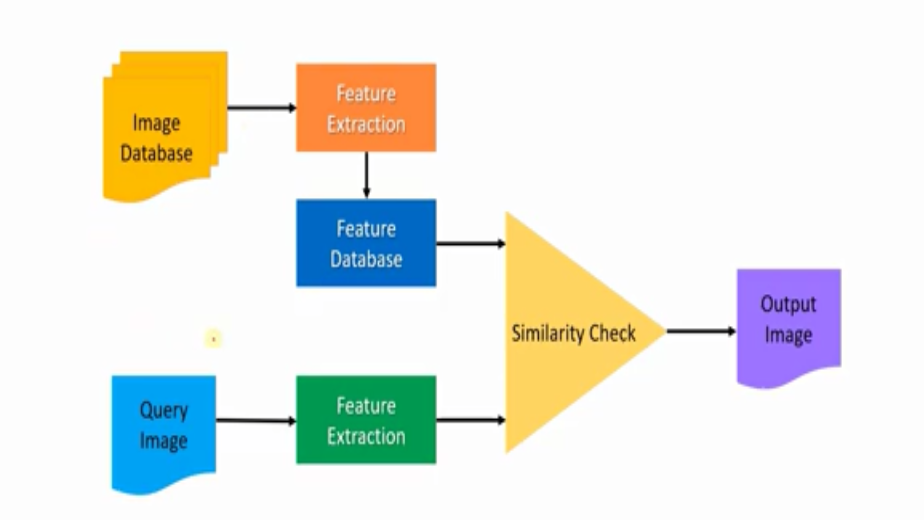
\includegraphics[width=120mm,height=60mm]{fig/19.png}
		\caption{image system block diagram }
		\label{image system block diagram}
	\end{figure}
	\begin{figure}[H]
	\centering
	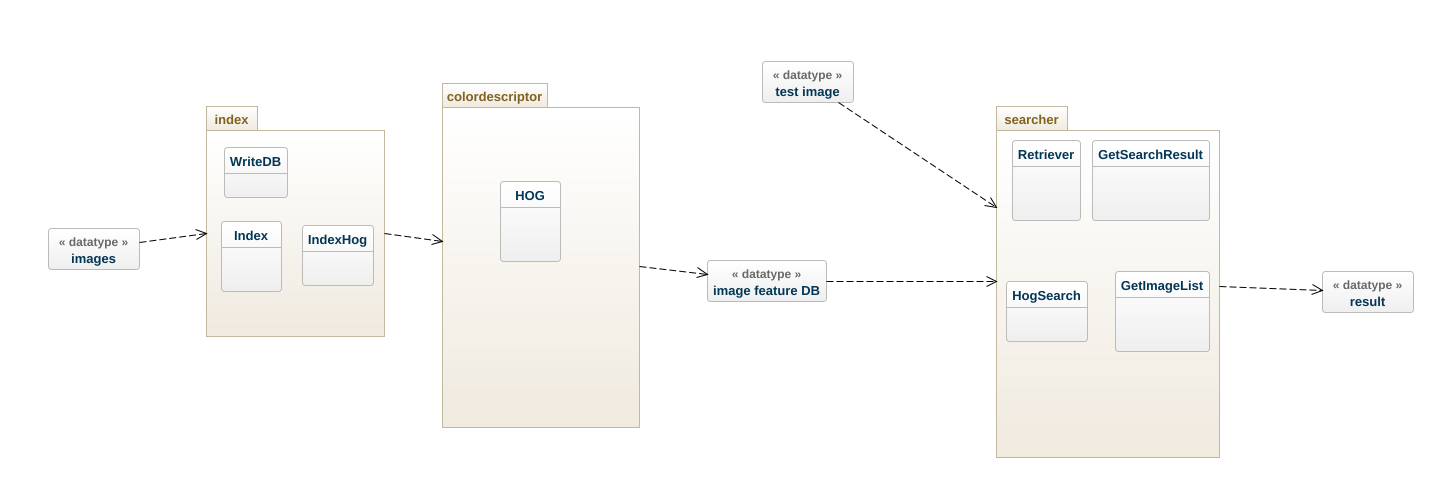
\includegraphics[width=120mm,height=60mm]{fig/22.png}
	\caption{video system block diagram }
	\label{video system block diagram}
\end{figure}
	\pagebreak
	\section{Beneficiaries of the project}
	The project is divided into two main parts CBIR and CBVR each can be beneficiaries for different groups.
	CBIR is helpful for Art Collections; painting can be searched by artists, moreover Medical images detecting tumors in medical scans, finally Satellite images for analysis or prediction.
	On other hand, CBVR is important in many fields such as Mass media used for search for videos of an incident, Forensic detecting person in other videos as the one you have and Surveillance Systems
	
	\pagebreak
	\section{Detailed analysis}
	This project deals with Content Based video Retrieval (CBVR)and Content Based Image Retrieval(CBIR). 
	For the CBIR, the adopted methods are color-based technique, texture-based technique, and shape-based technique. and then after the user select a technique and provide the image that he/she want to search for. The program extract features of the images dataset and save it then extract the features of the input image and compare the image with etracted feature database using the selected technique and by chi-squared distance. The chi-squared distance is distance measures that used to measures dissimilarity between two histograms. the following is an analysis for adopted technique in CBIR.
	\begin{enumerate}
		\item color based technique: searching for images using the color thy contain is widely used technique here we compute the distance based on the color using color histogram.
	
		\begin{figure}[H]
			\centering
			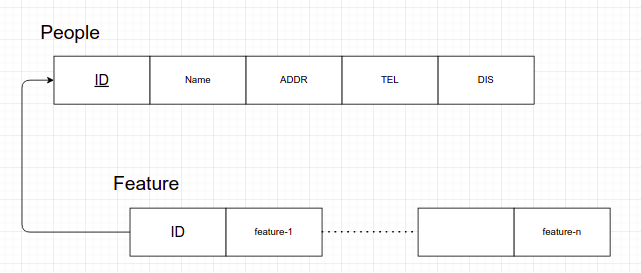
\includegraphics[width=120mm,height=60mm]{fig/24.png}
			\caption{color histogram  }
			\label{color histogram }
		\end{figure}
		\item texture based technique: in texture-based technique we search by the visual patterns in images. Here we use the gabour filter, it's a linear filter that used for texture analysis. we analysis the images if it has visual patterns match the image we search by.
		
		\item shape based technique: in shape-based technique we search for a shape of a specific region in the image. we extract features for shape based using the Histogram of Oriented Gradients (HOG). It's used in image processing for object detection.
	\end{enumerate}
some distance that we used to measure similarity 
\begin{itemize}
	\item Absolute Distance \\
	\begin{equation}
		D_{Absolute}(h,\bar{h})= \sum_{K-1}^{K} |h_{K}-\bar{h_{K}}|
	\end{equation}
	\item Euclidean Distance \\
	\begin{equation}
		D_{Euclidean}(h,\bar{h})= \sqrt{\sum_{K-1}^{K} (h_{K}-\bar{h_{K}})^{2}}
	\end{equation}
	\item Intersection Distance \\
	\begin{equation}
	D_{Intersection}(h,\bar{h})= 1- \sum_{K-1}^{K} in(h_{K},\bar{h_{K}})
	\end{equation}
	
	
	
\end{itemize}
in CBVR we used two techniques. the key frames extraction technique and content-based technique (Closed Captions).  The following is an analysis for adopted technique in CBIR.
\begin{enumerate}
	\item key frames extraction technique: by using key frames extraction technique you can retrieve video based on a given Frame. The video database created using features extraction of the key frames and then compare key frames features to the input Frame
	
	\item  Closed Captions: by using Closed Captions the user can search by a word or sentence in the .str or .vtt "the file format for Closed Captions" and find names of the videos that contain what he/she search for
\end{enumerate}

	
	\pagebreak
	\section{Detailed description of the adopted techniques }
	\subsection{Image}
	\begin{itemize}
		\item \textbf{{\large color based technique}} \\
		we use \textbf{mean color histogram} \\
		A histogram represents the distribution of pixel intensities as pins (whether color or grayscale) in an image. It can be visualized as a graph (or plot) that gives a high-level intuition of the intensity (pixel value) distribution. We are going to assume a RGB color space in this example, so these pixel values will be in the range of 0 to 255 then we get the mean values.
		Histogram matching can best be thought of as a “transformation.” Our goal is to take an input image (the “source”) and update its pixel intensities such that the distribution of the input image histogram matches the distribution of a reference image(in the data set).\\
		\textbf{{\large steps}}\\
		\begin{enumerate}
			\item We make picture to parts to make a better histogram
			\item Make histogram for each part
			\item Combine all histograms 
		\end{enumerate}
		\begin{figure}[H]
		\centering
		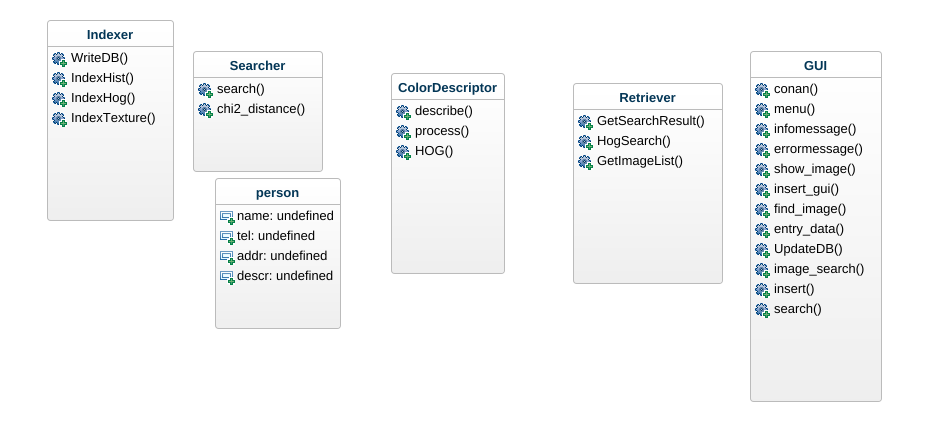
\includegraphics[width=120mm,height=60mm]{fig/23.png}
		\caption{color histogram similarity measure }
		\label{color histogram similarity measure}
	\end{figure}
	\item \textbf{{\large texture based technique}} \\
	we use \textbf{Gabour filter} \\
	The local structure of texture can be obtained by transforming a texture image to new basis given by convolving it with Gabor filters in order to segment images contain multiple textures\\
	\textbf{{\large steps}}\\
	\begin{enumerate}
		\item 	Turn the image to gray
		\item Create Gabour filters
		\item	Apply filters and choose the best 
		\item	Save features
		
	\end{enumerate}
\item \textbf{{\large shaped based technique}}\\
we use \textbf{histogram of gradient (HOG)} :\\
	The Histogram of Oriented Gradients (HOG) is a feature descriptor used in computer vision and image processing applications for the purpose of the object detection. It is a technique that counts events of gradient orientation in a specific portion of an image or region of interest. HOG focuses on the structure of the object. It extracts the information of the edges magnitude as well as the orientation of the edges.\\
\textbf{{\large steps}}\\
\begin{enumerate}
	\item (optional) global image normalization  applies an optional global image normalization equalization that is designed to reduce the influence of illumination effects
	\item	computing the gradient image in x and y computes first order image gradients. These capture contour, silhouette, and some texture information, while providing further resistance to illumination variations. 
	\item	computing gradient histograms produces an encoding that is sensitive to local image content while remaining resistant to small changes in pose or appearance. 
	\item	normalizing across blocks : computes normalization, which takes local groups of cells and contrast normalizes their overall responses before passing to next stage. Normalization introduces better invariance to illumination, shadowing, and edge contrast. 
\item	flattening into a feature vector  collects the HOG descriptors from all blocks of a dense overlapping grid of blocks covering the detection window into a combined feature vector
	
\end{enumerate}


	\end{itemize}
\subsection{video }
we use \textbf{thresholding} method(if difference between frames is greater than the thresholding value then it’s a key frame)  to extract key frames and  save the difference  between frames and the actual key frames\\
\textbf{{\large steps}}\\
\begin{enumerate}
	\item choose thresholding value
	\item	calculate difference between frames and compare it to thresholding value 
	\item	save difference and key frames
	
\end{enumerate}
	\textbf{video content(Text-based)}\\
	we use text-based retrieval using the text in the captions \\
	\begin{enumerate}
		\item choose a word or a sentence
		\item	search in the captions for all videos
		\item	return the videos that have the sentence
	\end{enumerate}
	
	\textbf{{\large distance}}\\
	we use Mean squared error method to compare between the image we search for and images saved in database 
	
	\pagebreak
	\section{Task breakdown structure}
		\begin{figure}[H]
		\centering
		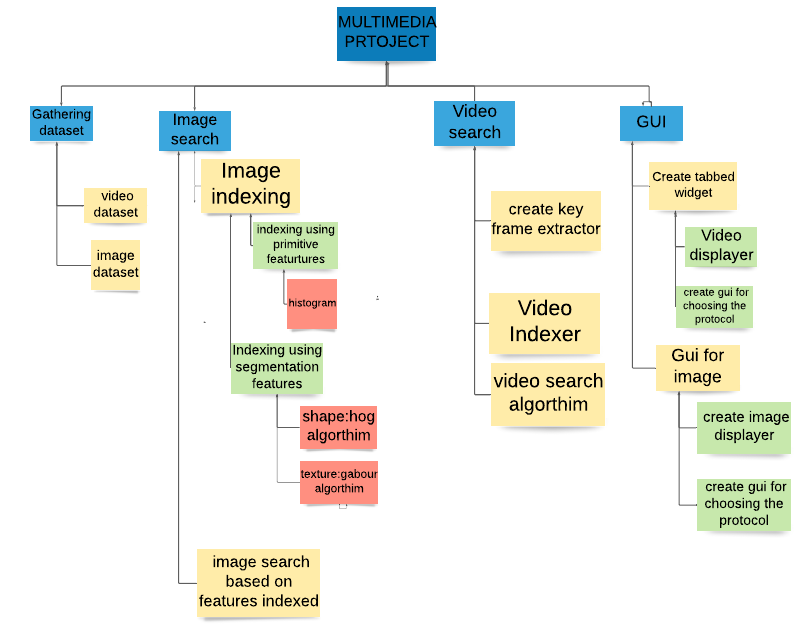
\includegraphics[width=140mm,height=160mm]{fig/25.png}
		\caption{WBS diagram}
		\label{WBS diagram}
	\end{figure}
	\pagebreak
	\section{Time plan}
	In Prepairing Datasets phase, We search for qualified dataset that qualify project. In parrallel, CBIR and CBVR Algorithms design  are finished. The software is developed from 11 to 25 April and then make testing for all functionality of the program.
	
	
	\begin{figure}[H]
		\centering
		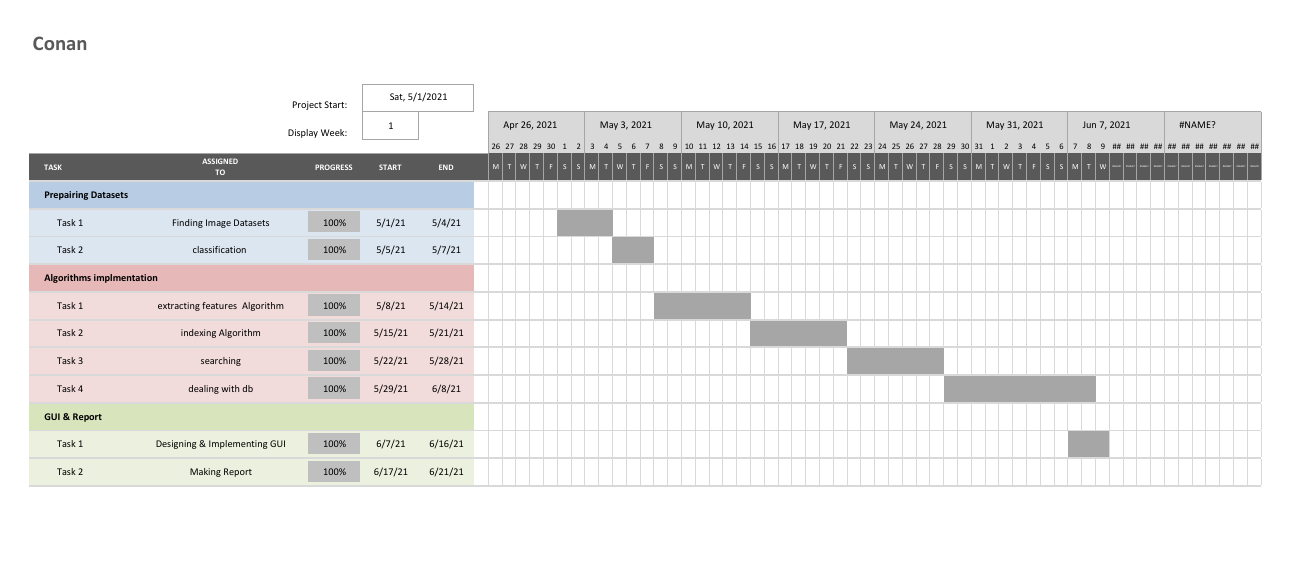
\includegraphics[width=140mm,height=80mm]{fig/5.png}
		\caption{time plan }
		\label{time plan}
	\end{figure}
	\pagebreak
	\section{System architecture}
	
	\begin{figure}[H]
		\centering
		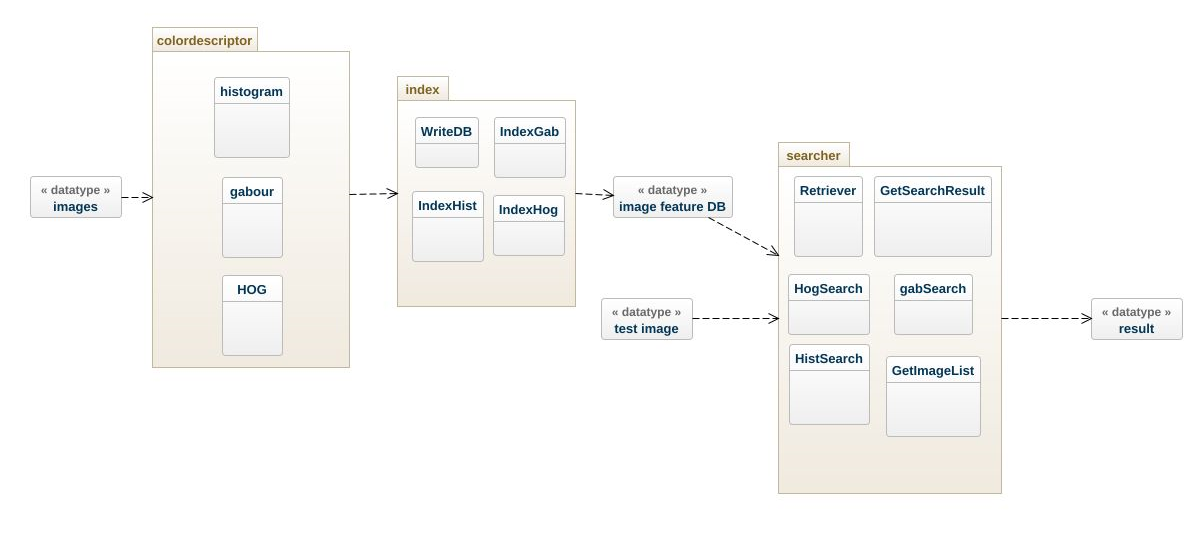
\includegraphics[width=120mm,height=60mm]{fig/0.png}
		\caption{image class diagram System}
		\label{image class diagram System}
	\end{figure}
\begin{figure}[H]
	\centering
	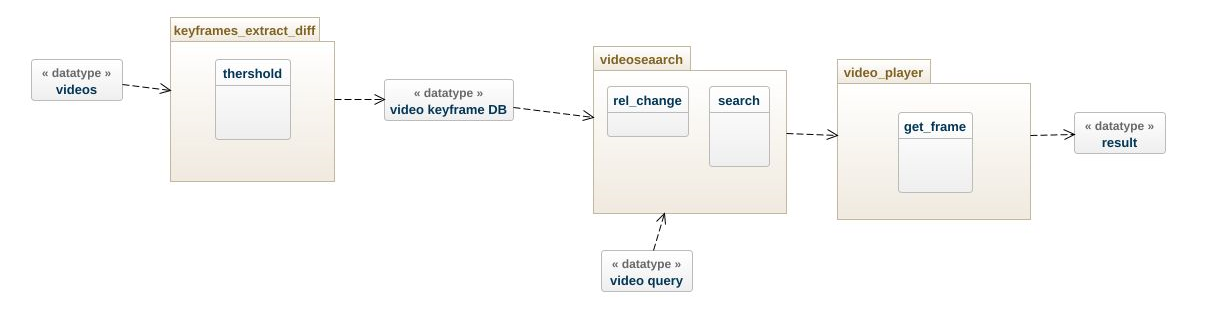
\includegraphics[width=120mm,height=60mm]{fig/1.png}
	\caption{video class diagram System  }
	\label{video class diagram System}
\end{figure}
\begin{figure}[H]
	\centering
	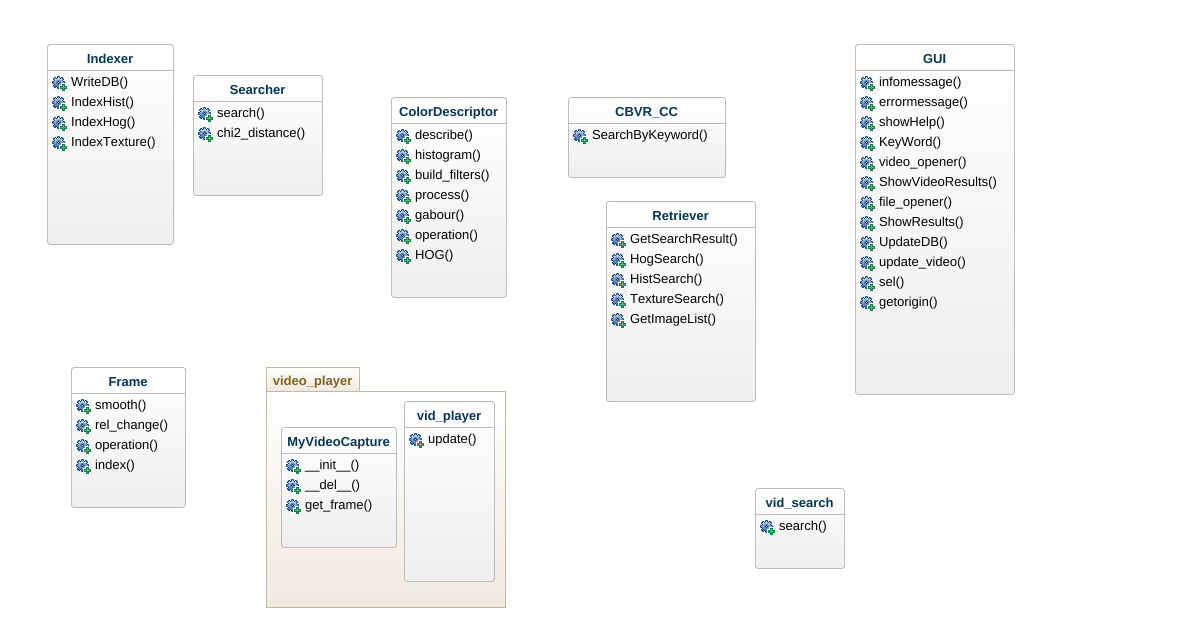
\includegraphics[width=140mm,height=120mm]{fig/33.png}
	\caption{class diagram }
	\label{class diagram }
\end{figure}
\pagebreak
	\section{Multimedia database design}
	\begin{figure}[H]
		\centering
		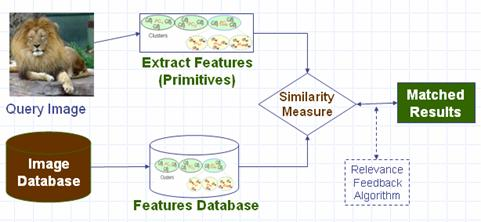
\includegraphics[width=120mm,height=60mm]{fig/18.png}
		\caption{extraction feature DB  }
		\label{extraction feature DB }
	\end{figure}
	we deal with diffrent types of media like photos videos metadata 
	so we include various extraction feture database in csv files like IndexHist.csv , IndexHog.csv , IndexShape.csv and video.csv
	we include diffrent types of dataset that used for testing and implmentation like 
	\begin{enumerate}
		\item CIFAR-10-images
		\item wang database
		\item microsoft image database
		\item Cambridge Object Recognition Image Database 
		\item 50 short clib
	\end{enumerate} 
\begin{figure}[H]
	\centering
	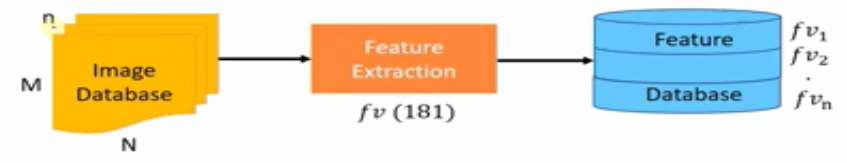
\includegraphics[width=120mm,height=60mm]{fig/21.png}
	\caption{image feature exract diagram }
	\label{image feature exract diagram}
\end{figure}
\begin{figure}[H]
	\centering
	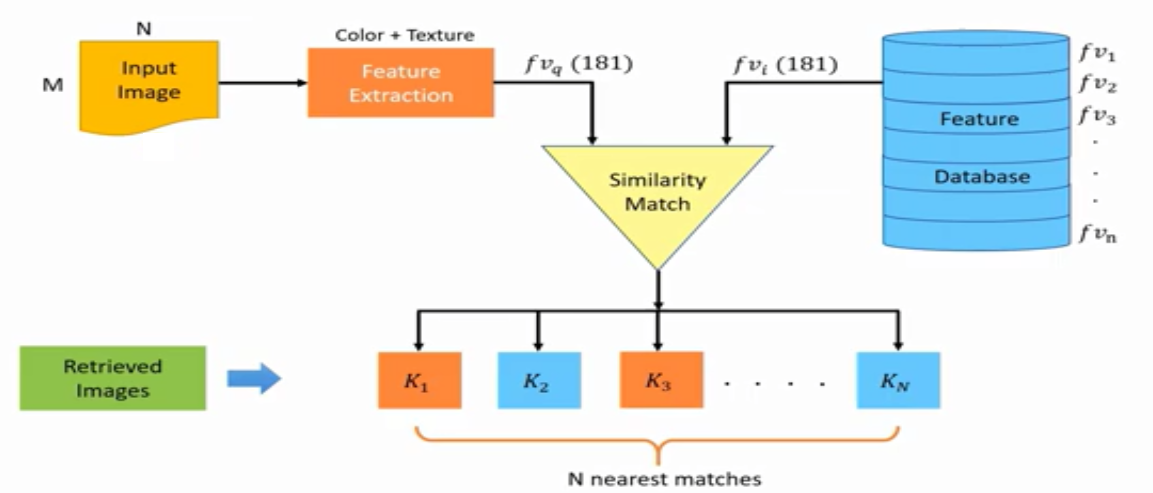
\includegraphics[width=120mm,height=60mm]{fig/20.png}
	\caption{image query diagram }
	\label{image query diagram}
\end{figure}
	\pagebreak
	\section{System design}
	\begin{enumerate}
		\item  \textbf{{\large system database}}\\
		in this project we have a database for CBIR which has a 3 CSV files each one store features for one technique.
		for CBVR. in key frames extraction we have a csv file which we store extracted key frames in it. for content-based "Closed Caption" we store the srt and vtt files on the disk
		
		\item \textbf{{\large user UI}} \\
		this is a GUI the user interact with to make queries.
		\item \textbf{{\large the processing part}}\\
		this part is responsible to process images and videos according to the selected technique.
		\item \textbf{{\large  operating scenario}}\\
		 first we build our database for video and images for all technique and then select from GUI video or image search if image user select the technique and the image want to search with. if video user enter the search keyword or the video want to search with. all data from GUI is passed to the processing part to give results and print it in the GUI  
		
	\end{enumerate}
	
	
	 
	
	
	
	\pagebreak
	\section{Testing scenarios and results}
	\subsection{CBIR}
	\begin{enumerate}
		\item Color Histogram \\
		The first algorithm implemented  in our project that relies on the color distribution of the image ,so images that have similar color distributions will be considered relevant to each other
		\begin{figure}[H]
			\centering
			\includegraphics[width=120mm,height=60mm]{fig/26.png}
			\caption{test image }
			\label{test image}
		\end{figure}
	Here see a blue sky and a brown sandy beach at the bottom and darkness from the shadow
	\begin{figure}[H]
		\centering
		\includegraphics[width=120mm,height=60mm]{fig/27.png}
		\caption{ Color Histogram test query result}
		\label{Color Histogram test query result}
	\end{figure}
So the results are the images that contain blue , brown or dark color as we see in image above
\item Shape Based\\
This algorithm is based on the Histogram of Oriented Gradients (HOG) is a feature descriptor for the purpose of the object detection. It is a technique that counts  gradient orientation in a specific portion of an image .\\
Here we have a photo of adel emam so when we use shape algorithm here are the results
	\begin{figure}[H]
		\centering
		\includegraphics[width=120mm,height=60mm]{fig/28.png}
		\caption{Shape Based test query result }
		\label{Shape Based test query result}
	\end{figure}
\item Texture Based\\
In this algorithm we  classify textures based on Gabor filter banks for edge detection. Frequency and orientation representations of the Gabor filter are similar to those of the human visual system
		\begin{figure}[H]
		\centering
		\includegraphics[width=120mm,height=60mm]{fig/29.png}
		\caption{Texture Based test query result}
		\label{Texture Based test query result}
	\end{figure}
	\end{enumerate}
\subsection{CBVR}
\begin{enumerate}
	\item Key Frame\\
	Here is the video we are looking for 
	\begin{figure}[H]
		\centering
		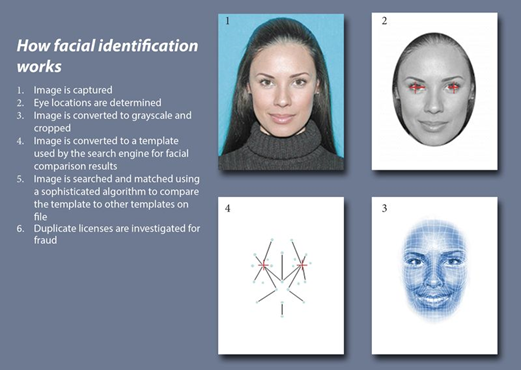
\includegraphics[width=120mm,height=60mm]{fig/30.png}
		\caption{test video }
		\label{test video}
	\end{figure}
so The video was found here in the result
\begin{figure}[H]
	\centering
	\includegraphics[width=120mm,height=60mm]{fig/31.png}
	\caption{video test query result }
	\label{video test query result}
\end{figure}
\pagebreak
\item Key word \\
To test this algorithm we have this line\\
“So let's dive into Flutter then and for this, let's create a brand new project. For that,”\\
Which is contained  in file named 018 Creating a New Project.en.srt , so if we try searching for this line here is the output
\begin{figure}[H]
	\centering
	\includegraphics[width=120mm,height=60mm]{fig/32.png}
	\caption{key word test query result }
	\label{key word test query result}
\end{figure}
\end{enumerate}
	\pagebreak
	\section{End user guide}
	\begin{enumerate}
		\item This is the primitive user interface.
		for choose the images services click on imagesearch tab or if needed to query for videos videosearch tab.
		
		\begin{figure}[H]
			\centering
			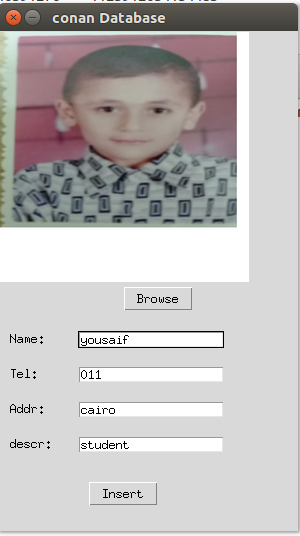
\includegraphics[width=120mm,height=60mm]{fig/6.png}
			\caption{imagesearch tab }
			\label{imagesearch tab}
		\end{figure}
				\begin{figure}[H]
			\centering
			
\includegraphics[width=120mm,height=60mm]{fig/8.png}
			\caption{videosearch tab }
			\label{videosearch tab}
		\end{figure}
	\pagebreak
	\item before to go in query we need to build database first so go from FILE chose updateImageDB
			\begin{figure}[H]
		\centering
		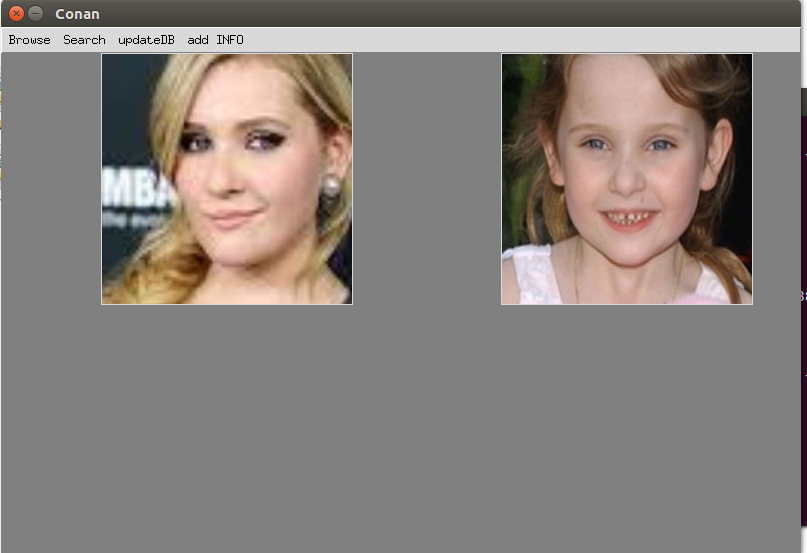
\includegraphics[width=120mm,height=60mm]{fig/10.png}
		\caption{updateImageDB }
		\label{updateImageDB}
	\end{figure}
	
		\item 	It may take a time and give you alert message for waiting.
\begin{figure}[H]
	\centering
	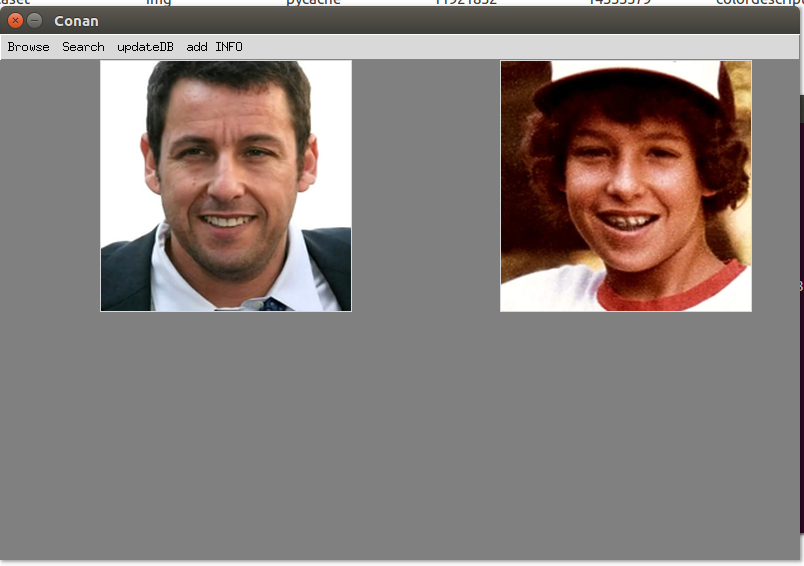
\includegraphics[width=120mm,height=60mm]{fig/12.png}
	\caption{waitting alert message }
	\label{waitting alert message}
\end{figure}
	
	
	\pagebreak
			\item 	When the database is finished updating, a message Database Status will appear.
	\begin{figure}[H]
		\centering
		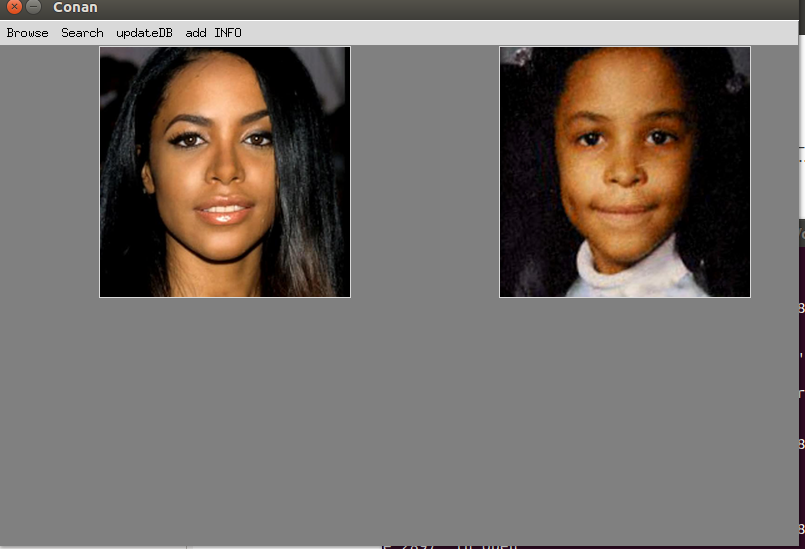
\includegraphics[width=120mm,height=60mm]{fig/13.png}
		\caption{updating finished message }
		\label{updating finished message}
	\end{figure}
	
	
	
	
	
	
	
	
		\item now we can search for any image we want From Browse choose Image ex Image of eyes and choose from Image Query the type of search you want like color based , texture based or shaped based. 
		
		\begin{figure}[H]
			\centering
			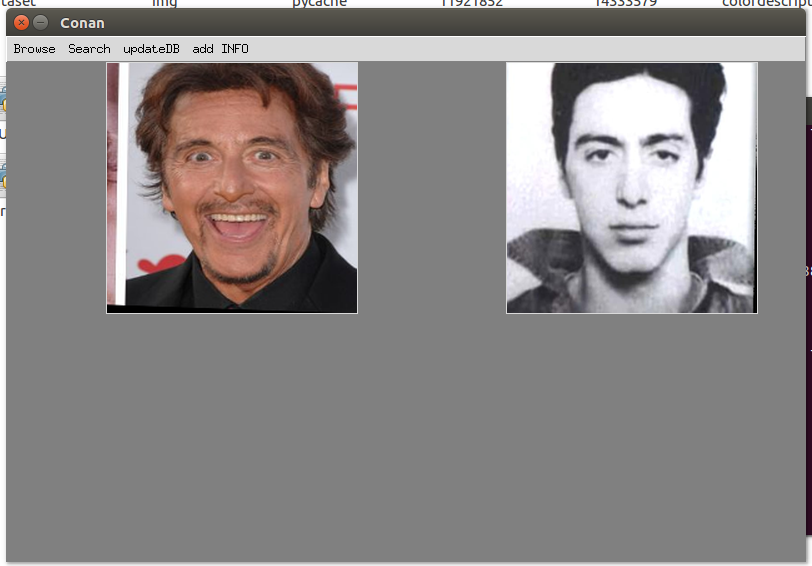
\includegraphics[width=120mm,height=60mm]{fig/11.png}
			\caption{image search task}
			\label{image search task}
		\end{figure}


\pagebreak
		\item 	to get the result Click on Retrieve button and the result will appear in the area for displaying results, and when you click at any result image it will be  standalone
		\begin{figure}[H]
			\centering
			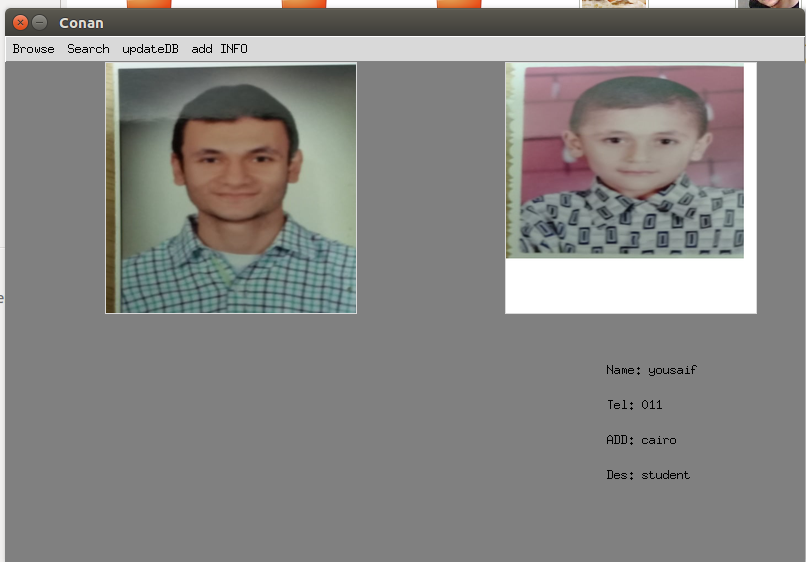
\includegraphics[width=120mm,height=60mm]{fig/14.png}
			\caption{image result task }
			\label{image result task}
		\end{figure}


	
	\item to begin search for videos we need first build video database
	so From file click on UpdateVideoDB.
		
		 
		\begin{figure}[H]
			\centering
			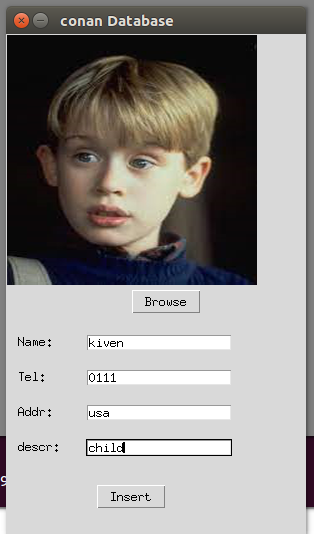
\includegraphics[width=120mm,height=60mm]{fig/9.png}
			\caption{UpdateVideoDB }
			\label{UpdateVideoDB}
		\end{figure}
	
	\pagebreak
		\item 	It may take a time and give you alert message for waiting.
	\begin{figure}[H]
		\centering
		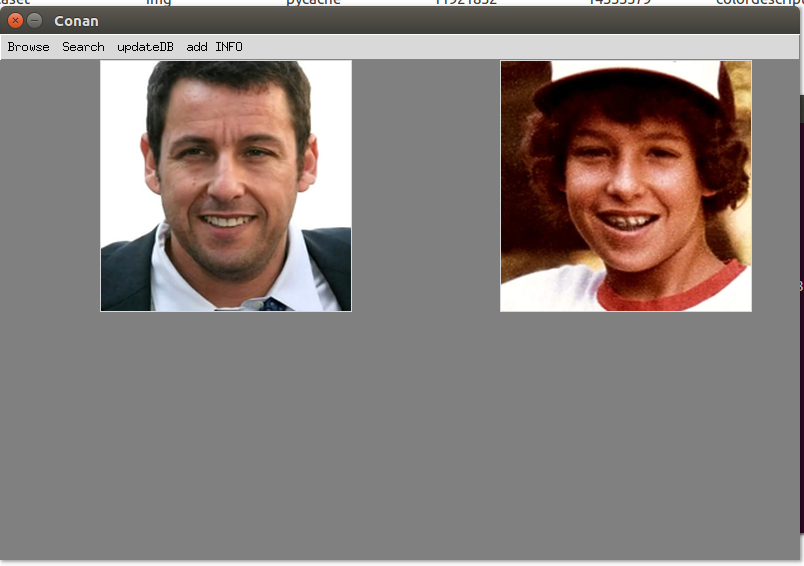
\includegraphics[width=120mm,height=60mm]{fig/12.png}
		%\caption{waitting alert message }
		%\label{waitting alert message}
	\end{figure}
	
	
	
	\item 	When the database is finished updating, a message Database Status will appear.
	\begin{figure}[H]
		\centering
		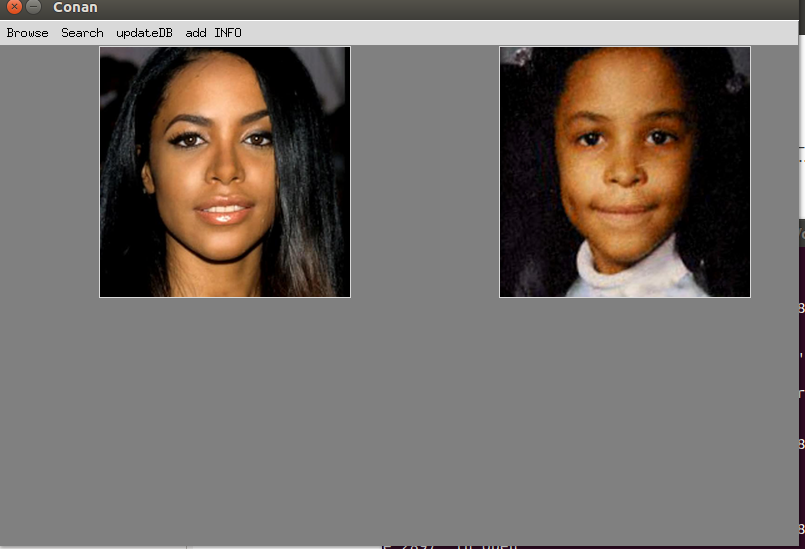
\includegraphics[width=120mm,height=60mm]{fig/13.png}
		%\caption{updating finished message }
		%\label{updating finished message}
	\end{figure}
\pagebreak
		\item to begin search task we can user either To search on the word belong video from subtitle or using keyframes 
		\begin{figure}[H]
			\centering
			
\includegraphics[width=120mm,height=60mm]{fig/8.png}
			%\caption{prime Gui }
			%\label{prime GUI}
		\end{figure}
	
	
		\item 	Write the Keyword you want to search it in the video in search By Keyword.
		\begin{figure}[H]
	\centering
	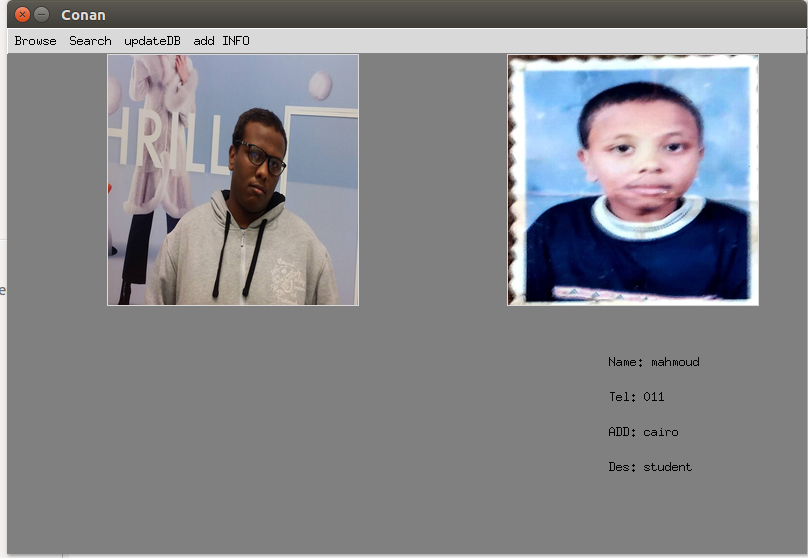
\includegraphics[width=120mm,height=60mm]{fig/16.png}
	\caption{search using keywords }
	\label{search using keywords}
\end{figure}

\pagebreak
		\item 	Click on keywords search and the result will appear in the result displaying.
\begin{figure}[H]
	\centering
	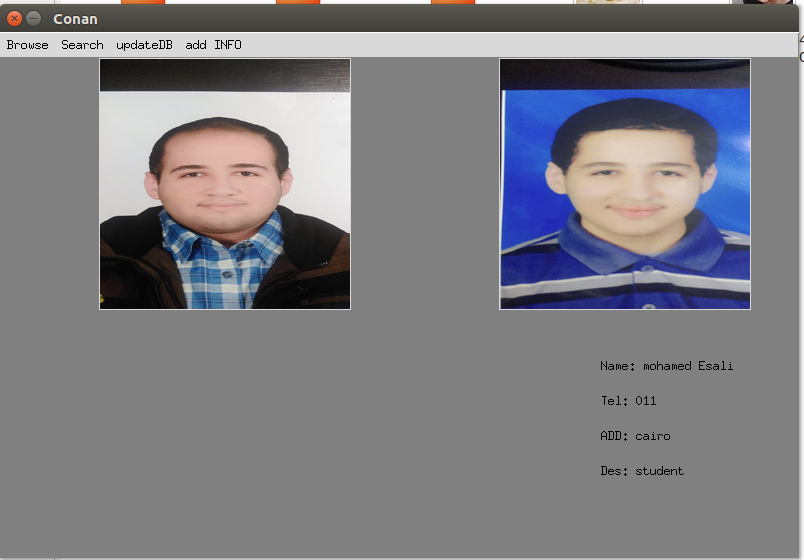
\includegraphics[width=120mm,height=60mm]{fig/15.png}
	\caption{keywords result  }
	\label{keywords result }
\end{figure}

		\item if we want to search using keyframes we click on video search tab and from browse chose the video.
				\begin{figure}[H]
			\centering
			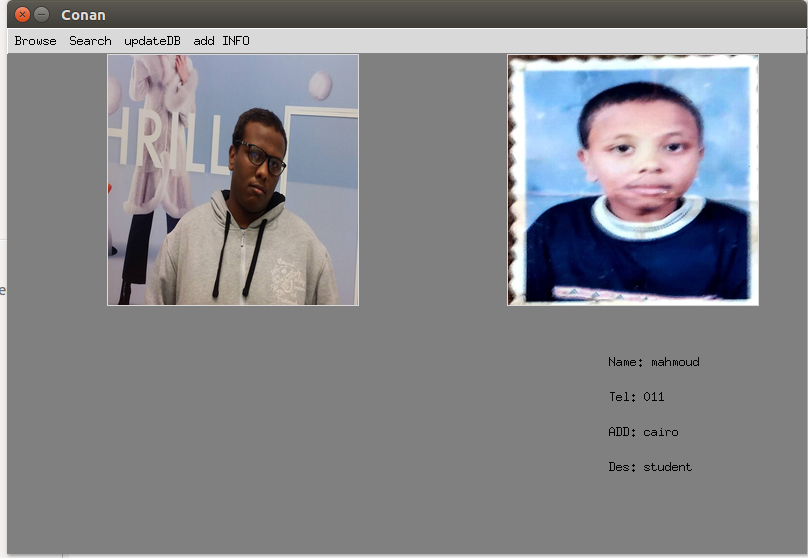
\includegraphics[width=120mm,height=60mm]{fig/16.png}
			\caption{search using keyframes }
			\label{search using keyframes}
		\end{figure}
		\pagebreak
				\item 	Click on Retrieve and the result will appear in the result displaying.
						\begin{figure}[H]
					\centering
					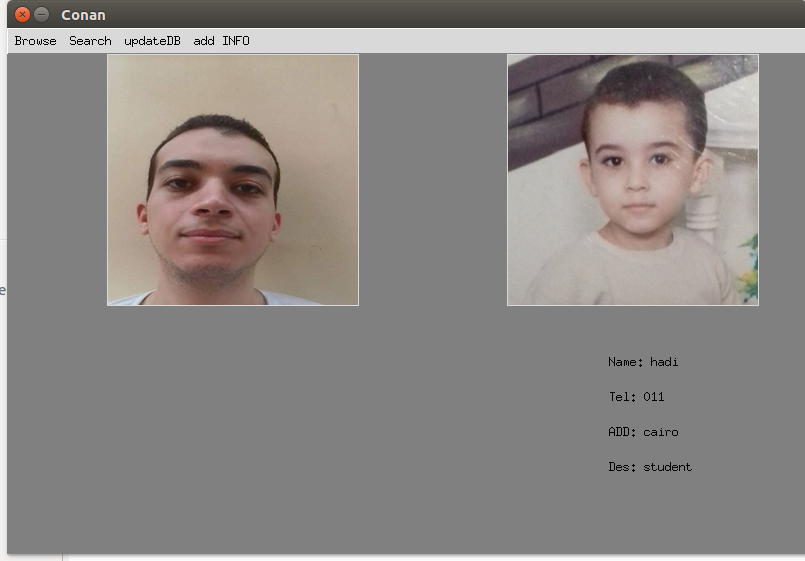
\includegraphics[width=120mm,height=60mm]{fig/17.png}
					\caption{keyframes results}
					\label{keyframes results}
				\end{figure}
	\end{enumerate}
\pagebreak
\section{Role of Each Member}
\begin{table}[H]
	\centering
	\begin{tabular}{||c| c ||} 
		\hline
		Name&Role\\[0.5ex] 
		\hline\hline
		ahmed Maged Abdel almonem& Task breakdown structure
		\\
		\hline
		Ahmed Mohammed Ibrahim& project description\\
		               &Beneficiaries of the project\\
		
		\hline
		 Bassem Mohamed Yousry&Testing scenarios and results\\
		 \hline
		 Mohamed Atta Ibrahim&System architecture \\
		                     &Multimedia database design \\
		 \hline
		 Mahmoud Mohamed Benyamin&Detailed description of the adopted techniques
		 \\
		 \hline
		 Mahmoud Othman Rabee & System design
		 \\
		 &Detailed analysis\\
		 
		 \hline
		  Hady Ashraf Ragab&Time plan\\
		                   &Conclusion
		                   \\
		  \hline
		  Yousef Abdelbadea Ali&Introduction\\
		  &End user guide
		  \\[1ex]
			\hline
	\end{tabular}
	\caption{Role of Each Member}
	\label{Role of Each Member}
\end{table}
	\pagebreak
	\section{Conclusion}
	
	At the end, the project can make a query by a query image using three CBIR algorithms such as (Gabour Filter, Histogram and Histogram of Gradient). It can make a query by a query video using only one CBVR algoritm such as (Extract Key Frame using Threshold). The user can use that project's program throw a friendly user interface (GUI), can choose between CBIR or CBVR, and can choose between those algorithms. The user can insert the query image or video and the results will appear to him/her.

	

	\pagebreak	
%	\addcontentsline{toc}{section}{References}
%	\bibliography{ref.bib} 
%	\bibliographystyle{ieeetr}
	
	
	\printglossary
\end{document}
